\documentclass[a4paper,12pt]{article}

\usepackage{graphicx}
\usepackage{graphics}
\usepackage{alltt}

\usepackage[dvips]{hyperref}
\title{Pararell and distribiuted programming}
\author{Author: Artur Skonecki \\ Scientific supervisor: Zuzanna Krawczyk}

\date{09/05/2013}

\begin{document}

\maketitle
\tableofcontents

\pagebreak
\section{Abstract}

This report outlines the design and development of a computer software
system for pararell XML xpath extraction from RSS feeds with support for a yet unknown database.
This program was written in Python to run under the Unix
operating system.


The design and ensuing program are modular
in nature (server-client architecture) and make maximum use of abstract data types and of software
re-use. Particular attention is paid to performance increase through pararellization
Client-server architecture provides the ability to use implemented features from any other program.


The report includes a full user manual, as well as the whole of the code that was written.
The source code was written with a particular focus on readability and clarity.

\section{Background}

Used technologies:
\begin{itemize}
 \item MPI - Message Passing Interface
 \item PyZMQ - ZeroMQ bindings for Python
 \item SqlAlchemy - generalized database access
 \item JSON - JavaScript Object Notation
\end{itemize}

\section{Design, implementation , and test setup}

The architecture.
\begin{center}
 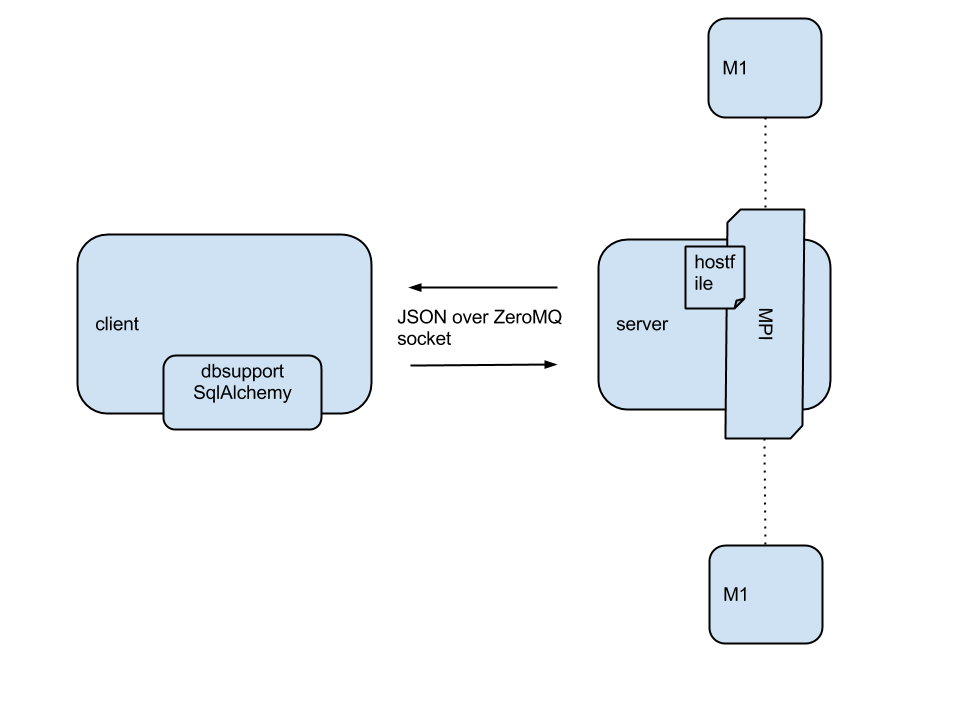
\includegraphics[width=\textwidth,height=\textheight,keepaspectratio]{prirdiagram.png}
 % prir diagram.png: 960x720 pixel, 72dpi, 33.87x25.40 cm, bb=0 0 960 720
\end{center}

\subsection{Data format}

  Format request sent by client to server (inludes authentication tokens: appid, appkey):
  \begin{verbatim}
  {
  "appid":appid,
  "appkey":appkey
  "url":url,
  "article_nums": article_nums,
  "xpath": xpath
  }
  \end{verbatim}
  
  Format of answers sent by server to client:

  \begin{verbatim}
  Reply format:
  {
  "article number' : list of extracted items,
  "article number' : list of extracted items,
  ...
  }
  \end{verbatim}
  
\subsection{server.py}

A program serving extracts of contents of articles in rss feed over zmq
sockets using json as data format.  This implementation uses MPI for
speeding up execution so it is taking advantage of concurrency features
of modern systems. Server requires authentication tokens appid and appkey.

\begin{verbatim}
server( port )
  Start a server listening for connections with zmq socket at 'port'
  for json requests from clients.

extract( xml, article_nums, xpath ) -> dict
  Return a dict containing article extracts.
\end{verbatim}




\subsection{client.py}

An implementation of a client:
\begin{itemize}
 \item request from server extracts of contents of articles in rss feed
 \item fetch the response
 \item write results to a dummy database:
 \begin{verbatim}
  TExtract( url, xpath, contents ) |one-to-many| TContent( content )
\end{verbatim}
 \item print out database
\end{itemize}

Uses json as data format.
ZeroMQ is deployed for communication between client and server.
SQLAlchemy for database access.


\begin{verbatim}
get_article_extracts( port, url, article_nums, xpath ) -> dict
  Return a dict containing rss article extracts.

main()
\end{verbatim}




\subsection{dbsupport.py}

A file containing classes implementing access to databases through SqlAlchemy.

\begin{verbatim}
class TExtract(Base)

class TContent(Base)

class DbSupport( object )
\end{verbatim}


%\verbatimfileinclude{client.py}
%\verbatimfileinclude{server.py}
%\verbatimfileinclude{dbsupport.py}

\section{Installation}
Install required packages on all hosts.
\begin{alltt}
apt-get install openmpi-bin libopenmpi-dev build-essentials python-dev python-zmq python-lxml python-sqlalchemy python-pip
pip install mpi4py
\end{alltt}

If server is supposed to run on multiple machines create a hostfile where server.py will be started.
The username should be the same on all machines. 4k2 directory should be the same on all machines.
\begin{alltt}
root@voyage:~/4k2# cat ~/hostfile
192.168.0.17
192.168.0.19
\end{alltt}



\section{Experiments}
Start server on a machine. Include hostfile if running on multiple machines.
\begin{alltt}
mpirun -np 4 --hostfile ~/hostfile python server.py
\end{alltt}

Extracting articles from a remote rss feed.
\begin{verbatim}
 python client.py \
-H 192.168.0.17 \
-f http://feeds.feedburner.com/TechCrunch \
-n 2,5,6,9,10 -s category[1]
\end{verbatim}

Example client output. 
\begin{verbatim}
Sending request {"url": "http://feeds.feedburner.com/TechCrunch",
  "xpath": "category[1]", "article_nums": [2, 5, 6, 9, 10]}
TExtract(u'http://feeds.feedburner.com/TechCrunch', 
  u'category[1]', [TContent(u'Fundings & Exits')])
TExtract(u'http://feeds.feedburner.com/TechCrunch', 
  u'category[1]', [TContent(u'Startups')])
TExtract(u'http://feeds.feedburner.com/TechCrunch', 
  u'category[1]', [TContent(u'Social')])
TExtract(u'http://feeds.feedburner.com/TechCrunch', 
  u'category[1]', [TContent(u'Enterprise')])
TExtract(u'http://feeds.feedburner.com/TechCrunch', 
  u'category[1]', [TContent(u'TC')])
\end{verbatim}



\section{Conclusion and future owrk}

Possible future directions:
\begin{itemize}
 \item authentication using OAuth
 \item tcp over ssl
\end{itemize}


\section{Code}

\subsection{client.py}
\begin{alltt}
\input{../client.py}
\end{alltt}

\subsection{server.py}
\begin{verbatim}
\input{../server.py}
\end{verbatim}

\subsection{dbsupport.py}
\begin{alltt}
\input{../dbsupport.py}
\end{alltt}


%\section{References}

%\section{Appendix}


% Background
% 
% Design, implementation , and test setup
% 
% Experiments
% 
% Conclusion and future owrk
% 
% References
% 
% Appendix
% 

\end{document}
